\documentclass[tikz,border=2pt]{standalone}
\usepackage{amsmath,amssymb}
\usepackage{pgfplots}
\pgfplotsset{compat=1.18}

\begin{document}
% The fundamental bridge: the indicator 1_A has mass 1 - P(A) at 0 and P(A) at 1, so its
% balance point (expectation) is exactly P(A). Probabilities are expectations of indicators.
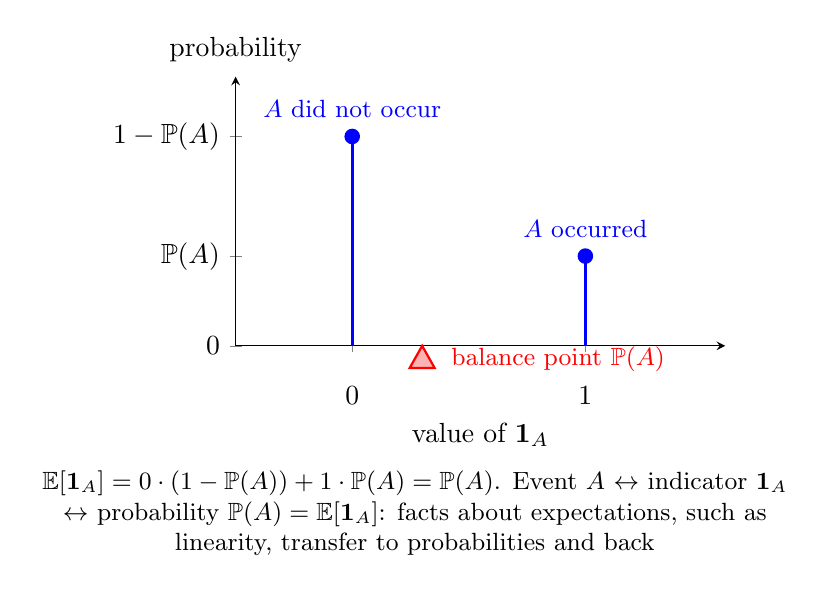
\begin{tikzpicture}
	\begin{axis}[
		axis lines=left, xmin=-0.5, xmax=1.6, ymin=0, ymax=0.9,
		xtick={0,1}, ytick={0,0.3,0.7}, yticklabels={$0$,$\mathbb{P}(A)$,$1-\mathbb{P}(A)$}, xticklabel style={yshift=-9pt},
		xlabel={value of $\mathbf{1}_A$}, ylabel={probability}, ylabel style={rotate=-90, anchor=south, at={(axis description cs:0,1.02)}},
		width=7.8cm, height=5cm, clip=false
		]
		\addplot[ycomb, blue, very thick, mark=*, mark size=2.2pt] coordinates {(0,0.7) (1,0.3)};
		\draw[red, thick, fill=red!30] (axis cs:0.3,0) -- ++(-4.5pt,-8pt) -- ++(9pt,0pt) -- cycle;
		\node[red, anchor=west, font=\small] at ([xshift=7pt,yshift=-5pt]axis cs:0.3,0) {balance point $\mathbb{P}(A)$};
		\node[blue, anchor=south, font=\small] at (axis cs:0,0.73) {$A$ did not occur};
		\node[blue, anchor=south, font=\small] at (axis cs:1,0.33) {$A$ occurred};
	\end{axis}
	\node[anchor=north, font=\small, align=flush center, text width=9.6cm] at ([yshift=-2pt]current axis.outer south) {$\mathbb{E}[\mathbf{1}_A]=0\cdot(1-\mathbb{P}(A))+1\cdot\mathbb{P}(A)=\mathbb{P}(A)$. Event $A$ $\leftrightarrow$ indicator $\mathbf{1}_A$ $\leftrightarrow$ probability $\mathbb{P}(A)=\mathbb{E}[\mathbf{1}_A]$: facts about expectations, such as linearity, transfer to probabilities and back};
\end{tikzpicture}
\end{document}
